\documentclass[a4paper,11pt]{article}
\usepackage{xeCJK}
\usepackage[margin=2cm]{geometry}
\usepackage{tikz}
\usetikzlibrary{positioning, shadows, calc}
\usepackage{amsmath,amssymb}
\usepackage{multicol}
\usepackage{enumitem}
\usepackage{fancyhdr}
\usepackage{xcolor}
\usepackage{mdframed}
\usepackage[most]{tcolorbox} % 使用 'most' 選項載入大部分函式庫
\usepackage{fontspec}
\usepackage{wrapfig}

% 指定本地字體路徑
\newfontfamily\sourcehansans{SourceHanSansTC-Regular}[
  Path=./assets/fonts/,
  Extension=.otf,
  BoldFont=SourceHanSansTC-Bold
]

% 設定中文字體 - 使用本地字體
\setCJKmainfont[
  Path=./assets/fonts/,
  Extension=.otf,
  BoldFont=SourceHanSansTC-Bold
]{SourceHanSansTC-Regular}

% 設定英文和數字字體
\setmainfont[
  Path=./assets/fonts/,
  Extension=.otf,
  BoldFont=SourceHanSansTC-Bold
]{SourceHanSansTC-Regular}

% 設定等寬字體 (如果有)
\setmonofont[
  Path=./assets/fonts/,
  Extension=.otf
]{SourceHanSansTC-Regular}

% 備用設定 - 如果您使用 Noto Sans CJK TC
% \setCJKmainfont[
%   Path=./assets/fonts/,
%   Extension=.otf,
%   BoldFont=NotoSansCJKtc-Bold
% ]{NotoSansCJKtc-Regular}

% 全局字體設置 - 增加行距
\renewcommand{\normalsize}{\fontsize{11pt}{18pt}\selectfont} % 增加行距
\renewcommand{\large}{\fontsize{14pt}{20pt}\selectfont}
\renewcommand{\Large}{\fontsize{16pt}{22pt}\selectfont}
\renewcommand{\huge}{\fontsize{20pt}{26pt}\selectfont}

% 設定頁面樣式
\pagestyle{fancy}
\fancyhf{}
\renewcommand{\headrulewidth}{0pt}
\fancyfoot[C]{\thepage}

% 設定段落間距 - 增加間距
\setlength{\parskip}{0.8em} % 增加段落間距
\setlength{\parindent}{0em}

% 設定列表樣式
\setlist[enumerate]{leftmargin=*,labelsep=0.5em,topsep=0.5em,itemsep=0.4em} % 增加列表項目間距

% 定義顏色
\definecolor{answerframe}{RGB}{120,120,120}
\definecolor{answerback}{RGB}{248,248,248}
\definecolor{explanationframe}{RGB}{70,130,180}
\definecolor{explanationback}{RGB}{240,248,255}
\definecolor{roundtitle}{RGB}{50,50,50}
\definecolor{accent6}{RGB}{52,73,94}

% Command for shadowed rounded rectangle question number
\newcommand{\qnumShadowBox}[1]{%
  \tikz[remember picture]{
    \node[rectangle, rounded corners=3pt, fill=white, draw=accent6, drop shadow, inner sep=2pt] (qnum) {\bfseries #1};
  }
}

% 答案盒子模板
\tcbset{
    answer/.style={
        enhanced,
        colback=answerback,
        colframe=answerframe,
        arc=2mm,
        boxrule=0.5pt,
        left=2mm
    }
}

% 答案列表環境
\newenvironment{answerraster}{%
    \begin{tcbraster}[
        raster columns=3,
        raster column skip=0.6cm, % 增加欄間距
        raster row skip=0.5cm, % 增加行間距
        raster left skip=0pt,
        raster right skip=0pt
    ]
}{%
    \end{tcbraster}
}

% 自定義環境
\newcommand{\answerbox}[2]{%
    \begin{tcolorbox}[
        answer,
        width=0.3\textwidth,
        text width=0.28\textwidth,
        title={#1}
    ]
        #2
    \end{tcolorbox}
}

% 定義 explanationbox 樣式 - 改善圖文排版
\tcbset{
    explanationstyle/.style={
        enhanced,
        breakable,
        colback=explanationback,
        colframe=explanationframe,
        arc=2mm,
        boxrule=0.5pt,
        fontupper=\fontsize{10.5pt}{16pt}\selectfont, % 增加字體大小和行距
        before skip=1.2em,
        after skip=1.2em,
        % 修正: 刪除 interior titled,改用下列選項
        title filled=true,
        colbacktitle=explanationframe,
        coltitle=white,
        toptitle=0.5mm,
        bottomtitle=0.5mm,
        top=8pt, % 增加內部上邊距
        bottom=8pt % 增加內部下邊距
    }
}

% 更新 explanationbox 命令,專門處理圖文混排
\newcommand{\explanationbox}[1]{%
  \begin{tcolorbox}[explanationstyle]
    #1
  \end{tcolorbox}
}

% 回標題樣式
\newcommand{\roundtitle}[1]{%
    \begin{center}
        \colorbox{roundtitle!10}{%
            \begin{minipage}{0.95\textwidth}
                \centering\large\textbf{\textcolor{roundtitle}{#1}}
            \end{minipage}
        }
    \end{center}
    \vspace{0.8em} % 增加標題下方間距
}

% 設定標題樣式
\usepackage{titlesec}
\titleformat{\subsection}
  {\normalfont\large\bfseries}{\thesubsection}{1em}{}
\titlespacing*{\subsection}{0pt}{2.5em}{1.5em} % 增加標題與內容間距

% 設定標題
\title{\huge 數學計算練習}
\author{\large 數學測驗生成器}
\date{\large \today}

% 調整 multicol 間距
\setlength{\columnsep}{1.5cm} % 增加欄間距

\begin{document}
\begin{center}
{\Large \textbf{數學計算練習 - 詳解}}
\end{center}

\noindent 生成日期:2025-04-28\hfill

\subsection*{第1回詳解}

\begin{multicols}{2}
\explanationbox{\textbf{1.} 
  \begin{minipage}{\linewidth}
    \begin{wrapfigure}{r}{0.45\linewidth}
      \centering 
      \vspace{-2em}
      \resizebox{3.5cm}{!}{
        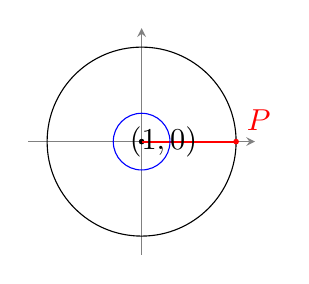
\begin{tikzpicture}[scale=1.2]
          % 子圖形 coordinates (類型: coordinate_system)
          \begin{scope}[shift={(0.0, 0.0)}]
            % 坐標系
            \usetikzlibrary{arrows.meta}
            
            \draw[-stealth, gray] (-1.2, 0) -- (1.2, 0);
            \draw[-stealth, gray] (0, -1.2) -- (0, 1.2);
          \end{scope}

          % 子圖形 circle (類型: circle)
          \begin{scope}[shift={(0.0, 0.0)}]
            % 圓形
            \draw[thin, solid, black] (0.0, 0.0) circle (1.0);
          \end{scope}

          % 子圖形 origin (類型: point)
          \begin{scope}[shift={(0.0, 0.0)}]
            % 點
            \fill[black] (0.0, 0.0) circle (0.03);
          \end{scope}

          % 子圖形 point (類型: point)
          \begin{scope}[shift={(0.0, 0.0)}]
            % 點
            \fill[red] (1.0, 0.0) circle (0.03) node[above right] {$P$};
          \end{scope}

          % 子圖形 radius (類型: line)
          \begin{scope}[shift={(0.0, 0.0)}]
            % 線段
            \draw[thin, thick, red] (0.0, 0.0) -- (1.0, 0.0);
          \end{scope}

          % 子圖形 angle (類型: angle)
          \begin{scope}[shift={(0.0, 0.0)}]
            % 角度
            \draw[thin, solid, blue] (0.0, 0.0) +(0.0:0.3) arc (0.0:360.0:0.3);
          \end{scope}

          % 子圖形 coord_label (類型: label)
          \begin{scope}[shift={(0.0, 0.0)}]
            % 標籤
            \node[left, black] at (0.7, 0.0) {$(1,0)$};
          \end{scope}
        \end{tikzpicture}
      }
      \vspace{-1.5em}
    \end{wrapfigure}
    \vspace{0.5em}
    因為 $\cot \theta = \frac{1}{\tan \theta} = \frac{x}{y}$,即 x 座標除以 y 座標。
    
    當 $\theta = 360^\circ$ 時,點的座標為 $(1, 0)$
    
    所以 $\cot(360^\circ) = \frac{1}{0} = \tilde{\infty}$
  \end{minipage}
}

\explanationbox{\textbf{2.} 
  \begin{minipage}{\linewidth}
    計算 $\tan^{-1}\left(\frac{\sqrt{2}}{2}\right)$:
    
    $\tan(35^\circ) = \frac{\sqrt{2}}{2}$
    
    但 $\tan^{-1}$ 的值域為 $(-90^\circ, 90^\circ)$
    
    因此 $\tan^{-1}\left(\frac{\sqrt{2}}{2}\right) = 35^\circ$
  \end{minipage}
}

\end{multicols}

\vfill
\begin{center}
\small{生成日期:2025-04-28}
\end{center}
\end{document}